\section{有限温度下的微扰论}

\subsection{推广的相互作用绘景}

推广的海森堡绘景下,算符可表示为($\hbar = 1$):

\begin{equation*}
O_K (\tau) = e^{K \tau} O_S e^{-K \tau}
\end{equation*}

这里: $K = H - \mu N$.


推广的相互作用绘景:

\begin{equation*}
O_I (\tau ) = e^{K_0 \tau} O_S e^{-K_0 \tau}
\end{equation*}

这里: $K_0 = H_0 - \mu N$, $K- K_0 = H - H_0 = H'$,
我们亦可用$O_I$来表示$O_S$,

\begin{equation*}
O_S = e^{-K_0 \tau} O_I (\tau) e^{K_0 \tau}
\end{equation*}

得到$O_K (\tau)$与$O_I (\tau)$之间的关系,

\begin{equation}\label{OK-OI-relation}
O_K(\tau) = e^{K \tau} e^{-K_0 \tau} O_I (\tau) e^{K_0 \tau}
e^{-K\tau}
\end{equation}

定义相互作用绘景下的演化算符为:

\begin{equation*}
U(\tau_1, \tau_2) = e^{K_0 \tau_1} e^{-K(\tau_1 - \tau_2)} e^{-K_0
\tau_2}
\end{equation*}

关系(\ref{OK-OI-relation})可改写为:

\begin{equation*}
O_K (\tau) = U(0, \tau) O_I (\tau) U(\tau, 0)
\end{equation*}

这里,

\begin{eqnarray*}
% \nonumber to remove numbering (before each equation)
  U(0,\tau) &=& e^{K\tau}e^{-K_0\tau} \\
  U(\tau,0) &=& e^{K_0 \tau} e^{-K\tau}
\end{eqnarray*}

必须指出的是$U$不是幺正算符, 即不满足$U^\dagger U =1$,
但$U$满足以下性质:

\begin{eqnarray*}
% \nonumber to remove numbering (before each equation)
  U(\tau_1, \tau_2) U(\tau_2, \tau_3) &=& U(\tau_1, \tau_3) \\
  U(\tau_1, \tau_1) &=& 1 \\
  U(\tau, 0)U(0, \tau) &=& U(0, \tau) U(\tau, 0) =  1
\end{eqnarray*}

推广的相互作用绘景下, 可求对$U$的偏导, $\frac{\partial U}{\partial
\tau}$,

\begin{equation}\label{time-evolution-of-U-tau}
\frac{\partial }{\partial \tau} U (\tau, 0) = - H'_I (\tau) U(\tau,
0)
\end{equation}

一阶微分方程, 存在形式解:

\begin{equation*}
U(\tau, 0) = 1 - \int_0^\tau d\tau_1 H'_I (\tau_1) U(\tau_1,0)
\end{equation*}

等式左右都有$U$, 反复迭代得到:

\begin{equation}\label{dyson-series-at-ft}
U(\tau,0) = \sum_{n=0}^\infty \frac{(-1)^n}{n!} \int_0^\tau d\tau_1
...\int_0^\tau d\tau_n T_\tau \left[ H'_I(\tau_1)...H'_I (\tau_n)
\right]
\end{equation}

考虑配分函数$e^{-\beta \Omega}$,

\begin{equation*}
e^{-\beta \Omega} = Tr e^{-\beta K} = Tr e^{-\beta K_0} e^{\beta
K_0} e^{-\beta K} = Tr \left[ e^{-\beta K_0} U(\beta , 0) \right]
\end{equation*}

利用迭代展开(\ref{dyson-series-at-ft}), 上式化为:

\begin{equation*}
e^{-\beta \Omega} = \sum_{n=0}^{\infty} \frac{(-1)^n}{n!}
\int_0^\beta d\tau_1 ... \int_0^\beta d\tau_n Tr \left[ e^{-\beta
K_0} T_\tau \left( H'_I(\tau_1)...H'_I(\tau_n) \right) \right]
\end{equation*}

回忆松原函数的定义, 仅写出$\tau > \tau'$的情形,

\begin{eqnarray*}
% \nonumber to remove numbering (before each equation)
  \mathcal{ G }_{\alpha, \beta}(x\tau,x'\tau') &=& - Tr \left\{e^{\beta(\Omega - K)} \psi_{K\alpha}(x\tau) \psi_{K\beta}^\dagger(x'\tau') \right\} \\
  {} &=& - e^{\beta \Omega} Tr \left\{ e^{-\beta K} \psi \psi^\dagger \right\} \\
  {} &=& - e^{\beta \Omega} Tr \left\{ e^{-\beta K_0} e^{\beta K_0} e^{-\beta K} ...
  \right\} \\
  {} &=& - e^{\beta \Omega} Tr \left\{ e^{-\beta K_0} U(\beta, 0) ...
  \right\}
\end{eqnarray*}

这里, $... = U(0,\tau) \psi_{I\alpha}(x\tau)U(\tau,0)U(0,\tau')
\psi_{I\beta}^\dagger(x'\tau') U(\tau',0)$.

因此,

\begin{equation*}
\mathcal{ G }_{\alpha\beta}(x\tau,x'\tau') = - \frac{ Tr \left\{
 e^{-\beta K_0} U(\beta,\tau) \psi_{I \alpha}(x \tau) U (\tau,\tau') \psi_{I \beta}^\dagger (x'\tau')U(\tau',0)  \right\} }{Tr \left\{ e^{-\beta K_0} U(\beta,0) \right\} }
\end{equation*}

即:

\begin{equation*}
\mathcal{ G }_{\alpha\beta}(x\tau,x'\tau') = - \frac{ Tr \left\{
 e^{-\beta K_0} T_\tau \left[ \psi_{I \alpha}(x \tau) \psi_{I \beta}^\dagger (x'\tau') U(\beta,0) \right] \right\} }{Tr \left\{ e^{-\beta K_0} U(\beta,0) \right\} }
\end{equation*}


引入记号$\left\langle ... \right\rangle_0 = Tr \left\{ e^{\beta
\Omega_0} e^{-\beta K_0} ... \right\}$,
即表示对无相互作用系统求热力学平均。


最终, 松原函数可写为:

\begin{equation*}
\mathcal{ G }_{\alpha\beta}(x\tau,x'\tau') = - \frac{\left\langle
T_\tau \left\{ \psi_{I\alpha}(x\tau)\psi_{I\beta}^\dagger (x'\tau')
U(\beta,0) \right\} \right\rangle_0  }{ \left\langle U(\beta, 0)
\right\rangle_0 }
\end{equation*}


\subsection{有限温度的维克定理}

类似于零温时的维克定理, 我们有:

\begin{equation}\label{wick th at ft}
\left\langle T_\tau (ABCD...) \right\rangle_0 = \sum_P (\mp)^P
\left\langle T_\tau(AB) \right\rangle_0 \left\langle T_\tau(CD)
\right\rangle_0 ...
\end{equation}


这里$P$表示的是所有``配对''方式,
$(\mp)^P$是不同算符``配对''引入的因子, 只对费米子有意义。
与零温时维克定理的区别是, 这里的$\left\langle ...
\right\rangle_0$是对无相互作用系统求的热力学平均,
而前者是对无相互作用系统求的基态(量子力学)平均。

我们可证明,

\begin{eqnarray*}
% \nonumber to remove numbering (before each equation)
  \left\langle T_\tau (\psi_{I\alpha}(x\tau) \psi_{I\beta}^\dagger (x'\tau')) \right\rangle_0 &=& - \mathcal{ G }_{\alpha \beta}^0 (x\tau, x'\tau') \\
  \left\langle T_\tau (\psi \psi) \right\rangle_0 &=& 0 \\
  \left\langle T_\tau (\psi^\dagger \psi^\dagger) \right\rangle_0 &=&
  0
\end{eqnarray*}


\subsection{有限温度的费曼图}

类似零温格林函数的讨论, 我们只需考虑连接图形:

\begin{equation*}
\mathcal{G}_{\alpha \beta}(x\tau,x'\tau') = - \left\langle T_\tau
\left\{ \psi_{I\alpha}(x\tau)\psi_{I\beta}^\dagger(x'\tau')
U(\beta,0) \right\} \right\rangle_c
\end{equation*}

...

回忆松原函数的傅立叶变换和逆傅立叶变换,

\begin{eqnarray*}
% \nonumber to remove numbering (before each equation)
  \mathcal{G}_{\alpha \beta}(x\tau) &=& \frac{1}{\beta} \sum_n \frac{1}{(2\pi)^3}\int d^3 p e^{ipx-i\omega_n \tau} \mathcal{G}_{\alpha \beta}(p,i\omega_n) \\
  \mathcal{G}_{\alpha \beta} (p,i\omega_n) &=& \int_0^\beta d \tau \int d^3 x  e^{-ipx + i \omega_n \tau} \mathcal{G}_{\alpha \beta} (x\tau)
\end{eqnarray*}

这里,

\begin{eqnarray*}
% \nonumber to remove numbering (before each equation)
  \omega_n &=& \frac{(2n+1)\pi}{\beta}, Fermions \\
  \omega_n &=& \frac{2n\pi}{\beta}, Bosons
\end{eqnarray*}

对无相互作用费米子, 我们曾经求得:

\begin{equation*}
\mathcal{G}_{\alpha \beta}^0 (p, i\omega_n) = \frac{\delta_{\alpha
\beta }}{i \omega_n - \epsilon_p^0 + \mu}
\end{equation*}

考虑相互作用:

\begin{equation}
V(x, \tau) = V(x_1 - x'_1)\delta(\tau_1 - \tau'_1) = \frac{1}{\beta} \sum\limits_n \frac{1}{(2\pi)^3}\int d^3 q e^{i (q x - \omega_n \tau)} V(q, \omega_n)
\end{equation}

这里:

\begin{equation}
\delta (\tau) = \frac{1}{\beta} \sum\limits_n e^{i \omega_n \tau} 
\end{equation}

(证明的思路是这样的:(1)当$\tau \neq 0$时,$\frac{1}{\beta} \sum\limits_n ... = 0 $;(2)当$\tau \to 0 $,$\frac{1}{\beta} \sum\limits_n ... \to \infty $;(3)积分:$ \frac{1}{\beta}  \int_0^{\beta}  d \tau (1 + e^{i \omega_1 \tau} +  e^{i \omega_2 \tau} + ... ) = 1 + 0 = 1 $。)

$\omega_n = \frac{2n \pi}{\beta}$, 导致:$V(q, \omega_n) = V(q)$,

\begin{eqnarray}
V(x)  &=&  \frac{1}{(2\pi)^3} \int d^3 q e^{i q x} V(q) \\
V(q) &=& \int d^3 x e^{-i q x} V(x)
\end{eqnarray}

对实空间画出费曼图,然后再做FT,对每一个内顶点都有能量-动量守恒。

\begin{equation}
\frac{1}{\beta} \int_0^{\beta} d \tau e^{i (\omega_n'' - \omega_n - \omega_n') \tau } = \delta_{\omega_n'' - \omega_n - \omega_n'}
\end{equation}

这里:$\omega_n$, $\omega_n''$ 是粒子线,$n$, $n''$可能取奇数,也可能取偶数,但其差一定取偶数。

$\omega_n'$ 是相互作用线,$n'$取偶数。

\subsubsection{动量空间的图形法则}

计算$\mathcal{G} (p, i \omega_n)$第n级贡献的费曼图形法则:

\begin{enumerate}
\item

画出n条相互作用线,2n+1条有向粒子线所有拓扑不等价连接图形。

为每一根相互作用线指定一个方向,并与一个波矢和分立的频率相联系。波矢和频率在每一个顶点上守恒。

\item

对费米子而言,$\omega_n = \frac{(2n +1)\pi}{ \beta}$。

\begin{equation*}
\mathcal{G}_{\alpha \beta}^0 (p, i\omega_n) = \frac{\delta_{\alpha
\beta }}{i \omega_n - \epsilon_p^0 + \mu}
\end{equation*}


对玻色子而言,$\omega_n = \frac{2n\pi}{ \beta}$。
 
\item

相互作用线振幅:$V(k, \omega_n) = V(k)$

\item

对所有独立的n个内波矢积分,对所有独立的n个内频率求和。

\begin{equation*}
\frac{1}{\beta} \sum\limits_n \frac{1}{(2 \pi)^3} \int d^3 p ...
\end{equation*}

\item 

任意连续的粒子线,对重复的自旋指标进行求和。

\item 

对F个闭合的费米圈(Fermion Loops),有附加的因子$(-1)^F$

总因子:

\begin{equation*}
(-1)^F \left[  \frac{-1}{\beta (2 \pi)^3} \right]^n
\end{equation*}

\item

粒子线自我闭合或被同一根相互作用线连接,需要插入收敛因子:$e^{i \omega_n \eta}$,$\eta$是无穷小的正量。

即粒子线的振幅是:

\begin{equation*}
\mathcal{G}^0_{\alpha \beta}  (p, i \omega_n) e^{i \omega_n \eta}
\end{equation*}

\end{enumerate}


\subsubsection{多费米系的一级图}

\begin{equation}
\mathcal{G}(k, \omega_n) = \mathcal{G}^0 (k, \omega_n) + \mathcal{G}^0 (k, \omega_n) \Sigma (k, \omega_n) \mathcal{G}^0  (k, \omega_n)   
\end{equation}

\begin{figure}[htbp]
\begin{center}
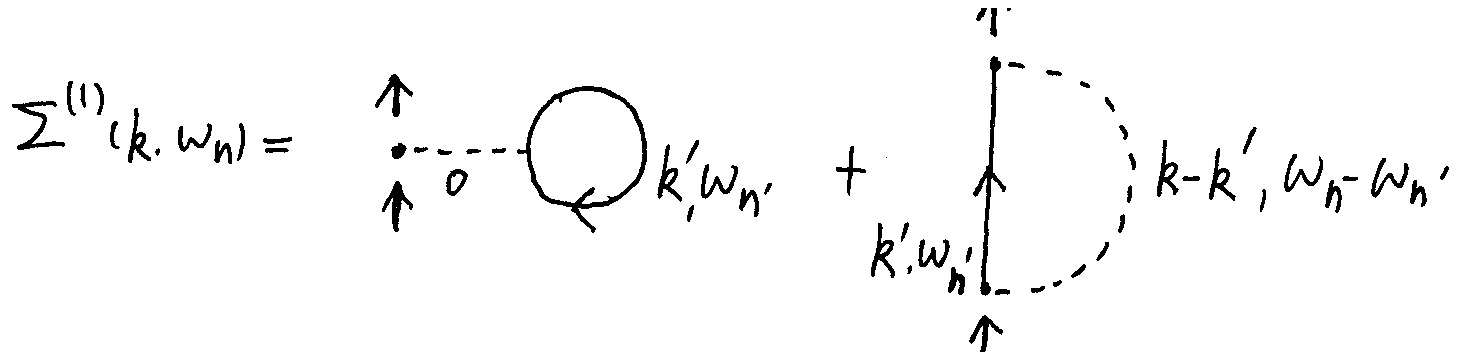
\includegraphics[width=10cm]{1stselfenergy.png}
\caption{一阶自能图}
%\label{default}
\end{center}
\end{figure}


写出$\Sigma^{(1)}(k, \omega_n)$

\begin{equation}
 - \frac{1}{\beta} \sum\limits_{n'} e^{i \omega_{n'} \eta} \int  \frac{d^3 k'} {(2 \pi)^3} \mathcal{G}^0 (k', \omega_{n'}) \left[ -(2s+1) V(0) + V(k - k')  \right]
\end{equation}

改写为:

\begin{equation*}
\int \frac{d^3 k'}{(2 \pi)^3} \left[ (2s+1) V(0) - V(k-k') \right] \cdot \frac{1}{\beta} \sum\limits_{n'} \frac{e^{i \omega_{n'} \eta} }{ i \omega_{n'}  - \epsilon_{k'} + \mu }
\end{equation*}

现在需要计算频率求和:

\begin{equation}
\frac{1}{\beta} \sum\limits_n e^{i \omega_n \eta} (i \omega_n - x )^{-1}
\end{equation}

可以证明:

\begin{equation}
\sum\limits_n \frac{ e^{ i \omega_n \eta } }{ i \omega_n - x } = \mp \frac{\beta}{  e^{\beta x} \mp 1 }
\end{equation}

“-”是玻色子,“+”是费米子。

因此:

\begin{equation}
\Sigma^{(1)}(k) = \int \frac{d^3 k'}{(2 \pi)^3} \left[ (2s+1)V(0) - V(k - k') \right] n^0_{k'}
\end{equation}

这里,费米子的$n^0_{k'}$

\begin{equation}
n^0_{k'} = \frac{1}{ e^{ \beta ( \epsilon^0_{k'} - \mu  ) } + 1 }
\end{equation}

\subsection{频率求和}

\subsubsection{费米子的频率求和}

考虑费米子,$\omega_n = \frac{ (2n+1) \pi}{\beta}$,求证:

\begin{equation}
\sum\limits_{n \in odd } \frac{e^{i \omega_n \eta}}{i \omega_n - x } =\frac{ \beta}{ e^{\beta x} + 1 }
\end{equation}

证:

考虑复函数:

\begin{equation}
f(z) = \frac{1}{e^{\beta z} + 1}
\end{equation}

$f(z)$在复平面上奇点的位置:$\beta z = i (2n +1) \pi$,即:

\begin{equation*}
z = i \omega_n = \frac{i (2n +1)\pi }{\beta}
\end{equation*}

在这些奇点上$f(z)$的留数是:

\begin{equation*}
\lim\limits_{z \to i\omega_n  } \frac{z - i \omega_n}{ e^{\beta z} + 1 } =  \lim\limits_{z \to i\omega_n  } \frac{1}{ \beta e^{\beta z}  } = - \frac{1}{\beta}
\end{equation*}

这里利用了“罗比达”法则:$\lim\limits_{z \to z_0} \frac{f(z)}{g(z)} = \lim\limits_{z \to z_0} \frac{ f'(z) }{ g'(z) } $

\begin{figure}[htbp]
\begin{center}
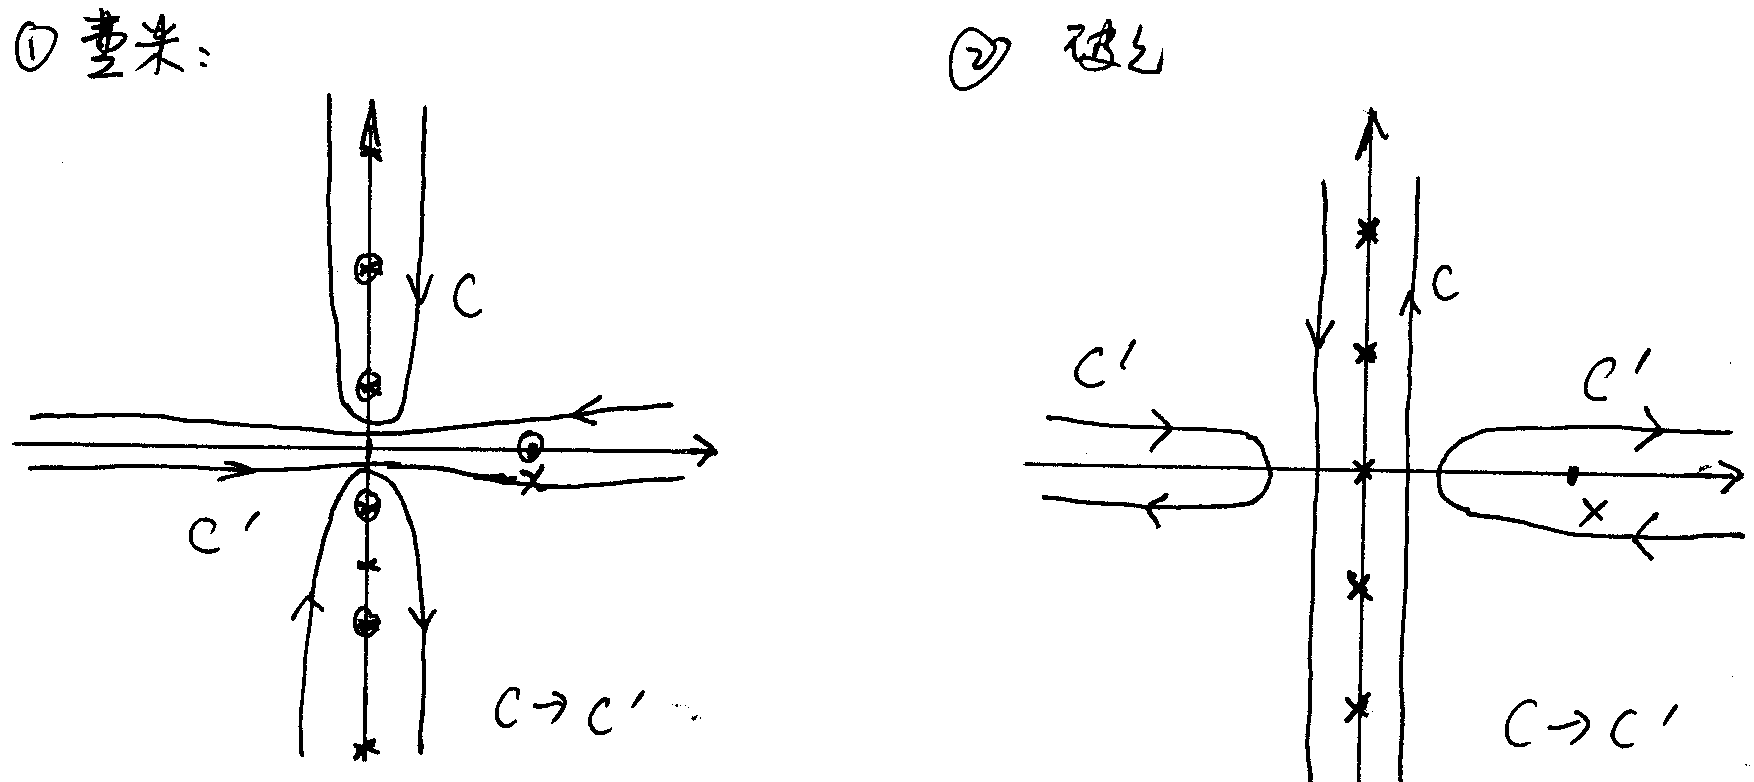
\includegraphics[width=10cm]{Finite/frequencysummation.png}
\caption{频率求和}
%\label{default}
\end{center}
\end{figure}

考虑积分:

\begin{equation*}
\frac{1}{2\pi i} \int_C \frac{ dz e^{z \eta} }{z -x} f(z)
\end{equation*}

这个积分的奇点有:(1)$z = x$,在实轴上;(2)$z = i \omega_n$,在虚轴上的奇数格点。

积分回路C是顺时针的,总体会有一个“-”,但会与留数$- \frac{ 1 }{\beta} ...$的“-”抵消。积分回路C'是逆时针的。

最终结果是:

\begin{equation}
\frac{1}{\beta} \sum\limits_n \frac{e^{i \omega_n \eta}}{ i \omega_n - x} = f(x) = \frac{1}{e^{\beta (\epsilon_k - \mu)} + 1 }
\end{equation}


\subsubsection{玻色子的频率求和}

考虑玻色子,$\omega_n = \frac{2n \pi}{\beta}$,求证:

\begin{equation}
\sum\limits_{n \in even} \frac{e^{i \omega_n \eta}}{i \omega_n - x } =\frac{- \beta}{ e^{\beta x} - 1 }
\end{equation}

证:

考虑复函数:

\begin{equation}
f_B (z)  = \frac{1}{e^{\beta z}  -1}
\end{equation}

奇点位置$z = i \omega_n$,$\omega_n = \frac{2n \pi}{ \beta}$

$f_B(z)$在$i \omega_n$处的留数:

\begin{equation*}
\lim\limits_{z \to i \omega_n}  \frac{z - i \omega_n}{ e^{\beta z }  - 1 } = \frac{(...)'}{(...)'} = \frac{1}{\beta}
\end{equation*}

构造积分:

\begin{equation}
\frac{1}{2 \pi i } \int_C \frac{dz e^{z \eta}} { z -x }
\end{equation}

积分回路C是逆时针的;积分回路C'是顺时针的,因此有一个额外的“-”。

因此:

\begin{equation*}
\frac{1}{\beta} \sum\limits_n \frac{ e^{i \omega_n \eta} } { i \omega_n - x } = - f_B (x) = - \frac{1}{e^{ \beta(\epsilon_k - \mu )} -1 }
\end{equation*}
